% desafiofinal.tex
\section{Desafío Final: Implementación y Explicación}

\subsection{Crear Código Assembler para Pasar a Modo Protegido (sin macros)}

El objetivo era crear un sector de arranque (MBR) que, iniciando en Modo Real de 16 bits, realizara los pasos necesarios para entrar en Modo Protegido de 32 bits utilizando las instrucciones máquina explícitas, sin depender de macros que pudieran ocultar el proceso.

\subsubsection{Estructura del Código y Archivos}

Para una mejor organización y reutilización, el código se dividió en varios archivos fuente ensamblador (usando sintaxis NASM):
\begin{itemize}
    \item \texttt{pm.asm}: Archivo principal que contiene el punto de entrada (\texttt{\_start}), la inicialización básica, las llamadas a las funciones de impresión y transición, y las definiciones de mensajes.
    \item \texttt{print\_string.asm}: Contiene la función \texttt{print\_string} para imprimir cadenas en Modo Real usando la interrupción 0x10 del BIOS.
    \item \texttt{gdt.asm}: Define la Tabla de Descriptores Globales (GDT) necesaria para el Modo Protegido, incluyendo el descriptor nulo obligatorio, un descriptor para el segmento de código y un descriptor para el segmento de datos. También define el descriptor especial que apunta a la propia GDT (requerido por la instrucción \texttt{lgdt}).
    \item \texttt{switch\_to\_pm.asm}: Contiene la función \texttt{switch\_to\_pm} que ejecuta la secuencia de transición (deshabilitar interrupciones, cargar GDT, activar bit PE en CR0, salto largo) y la etiqueta \texttt{init\_pm} donde aterriza el código de 32 bits para configurar los segmentos y la pila en Modo Protegido.
    \item \texttt{print\_string\_pm.asm}: Contiene la función \texttt{print\_string\_pm} para imprimir cadenas directamente en la memoria de video (\texttt{0xB8000}), necesaria ya que el BIOS no está disponible en Modo Protegido.
\end{itemize}
El archivo principal \texttt{pm.asm} utiliza la directiva \texttt{\%include} de NASM para incorporar el contenido de los otros archivos durante el ensamblaje.

\subsubsection{El Problema del Formato Binario Directo (\texttt{-f bin})}

Inicialmente, se intentó ensamblar directamente a un formato binario crudo usando \texttt{nasm pm.asm -f bin -o pm.img}. Sin embargo, este enfoque presentó serios problemas al depurar con GDB:
\begin{itemize}
    \item \textbf{Desensamblado Incorrecto:} GDB mostraba secuencias de instrucciones inválidas (\texttt{(bad)}) o incorrectas en direcciones donde se esperaba código válido (especialmente después de los \texttt{call} o cerca de los límites de los archivos incluidos).
    \item \textbf{Fallo Prematuro (Triple Fallo):} La ejecución en QEMU fallaba catastróficamente (probablemente por un Triple Fallo) justo al intentar realizar el salto largo (\texttt{ljmp}) a Modo Protegido, indicando que la CPU no podía encontrar o validar el descriptor de código especificado o la dirección de destino.
\end{itemize}
La causa raíz es que NASM, al generar un binario crudo (\texttt{-f bin}) a partir de múltiples archivos incluidos y con cambios de modo (\texttt{[bits 16]}, \texttt{[bits 32]}), no tiene suficiente información contextual para calcular y colocar correctamente todos los offsets, direcciones y bloques de código/datos relativos a la dirección de carga final (\texttt{0x7C00}) y resolver referencias entre los diferentes «módulos» incluidos. El resultado era un archivo \texttt{pm.img} corrupto o mal estructurado.

\subsubsection{Solución: Flujo de Trabajo ELF}

Para solucionar estos problemas, se adoptó un flujo de trabajo más robusto y estándar utilizando un formato intermedio:
\begin{enumerate}
    \item \textbf{Ensamblar a ELF:} Se ensambló el archivo principal \texttt{pm.asm} (que incluye a los demás) a un formato de objeto ELF de 32 bits usando \texttt{nasm -f elf pm.asm -o pm.o}. ELF (Executable and Linkable Format) es un formato que preserva la información sobre secciones (\texttt{.text}, \texttt{.data}), símbolos (etiquetas como \texttt{\_start}, \texttt{print\_string}, \texttt{gdt\_start}), y datos de relocalización necesarios para el linker.
    \item \textbf{Enlazar con LD y Script:} Se utilizó el linker GNU \texttt{ld} con la opción \texttt{-m elf\_i386} (para asegurar compatibilidad con el objetivo i386) y un script de linker (\texttt{link.ld}). Este script instruye a \texttt{ld} para:
        \begin{itemize}
            \item Establecer la dirección de carga base en \texttt{0x7C00}.
            \item Combinar las secciones \texttt{.text}, \texttt{.data}, etc., del archivo \texttt{pm.o} en una única sección de salida posicionada en \texttt{0x7C00}.
            \item Resolver todas las direcciones (como la dirección de \texttt{gdt\_start} usada por \texttt{lgdt}, la dirección de \texttt{MSG\_REAL\_MODE} usada por \texttt{mov si}, y las direcciones de las funciones \texttt{print\_string} y \texttt{switch\_to\_pm} usadas por \texttt{call}) relativas a la base \texttt{0x7C00}.
            \item Asegurar que el archivo de salida tenga exactamente 512 bytes, añadiendo relleno si es necesario y la firma MBR \texttt{0xAA55} al final (usando \texttt{. = 0x7C00 + 510; BYTE(0x55) BYTE(0xAA);}).
        \end{itemize}
        Comando: \texttt{ld -m elf\_i386 -T linker.ld -o pm.elf pm.o}
\end{enumerate}
Este enfoque delega la compleja tarea de posicionamiento y resolución de direcciones al linker (\texttt{ld}), que está diseñado específicamente para ello, resultando en un archivo \texttt{pm.img} correctamente estructurado y funcional.

\subsubsection{Código de Transición Detallado (en \texttt{switch\_to\_pm.asm})}

El núcleo de la transición reside en la función \texttt{switch\_to\_pm}, que realiza los siguientes pasos indispensables (sin macros):

\newpage

\begin{lstlisting}[style=NasmStyle, breaklines=true,
    caption={\texttt{switch\_to\_pm.asm} (Nucleo de la transicion)}]
[bits 16]
switch_to_pm:
cli                         ; 1. Deshabilitar interrupciones enmascarables.
                            ;    para evitar que una IT ocurra durante la transicion
                            ;    cuando el estado de la CPU es inconsistente.

lgdt [gdt_descriptor]       ; 2. Cargar el Registro Descriptor de la GDT (GDTR).
                            ;    Lee 6 bytes desde la direccion de la etiqueta 'gdt_descriptor'.
                            ;    Esos 6 bytes contienen el limite (tamanio-1) de la GDT
                            ;    y la direccion base lineal donde reside la GDT en memoria.
                            ;    Esto informa a la CPU donde encontrar la tabla GDT.

; 3. Activar Modo Protegido (Bit PE en CR0)
mov eax, cr0                ; 3a. Leer el registro de control CR0 en EAX (32 bits).
or eax, 0x01                ; 3b. Poner el bit 0 (PE - Protection Enable) a 1 usando OR.
                            ;     Los otros bits de CR0 se mantienen.
mov cr0, eax                ; 3c. Escribir el valor modificado de vuelta a CR0.
                            ;     A partir de este instante, la CPU opera en Modo Protegido.

; 4. Salto Largo (Far Jump)
;    Es OBLIGATORIO inmediatamente despues de activar PE. Sirve para:
;    a) Limpiar la cola de prefetch de instrucciones de la CPU, que podria
;       contener instrucciones decodificadas como si fueran de Modo Real.
;    b) Cargar el registro de segmento de Codigo (CS) con un SELECTOR valido
;       de nuestra nueva GDT.
;    c) Transferir la ejecucion al codigo disenado para 32 bits.
jmp 0x08 : init_pm          ; Salto a: Selector de Codigo (0x08, segundo descriptor)
                            ;          Offset (direccion de la etiqueta 'init_pm')

[bits 32]                   ; A partir de aqui, el ensamblador genera codigo de 32 bits
init_pm:                    ; Punto de aterrizaje en Modo Protegido
; 5. Configurar Segmentos de Datos y Pila (32 bits)
mov ax, 0x10                ; Cargar SELECTOR del segmento de Datos (0x10) en AX.
                            ; Se usa AX (16 bits) porque los selectores son de 16 bits.
mov ds, ax                  ; Cargar DS con el selector de datos.
mov ss, ax                  ; Cargar SS (segmento de pila) con el mismo selector.
mov es, ax                  ; Cargar ES.
mov fs, ax                  ; Cargar FS (opcional).
mov gs, ax                  ; Cargar GS (opcional).
; Ahora todos los accesos a datos o pila usaran el descriptor GDT en el indice 2.

; 6. Configurar el Puntero de Pila (ESP)
mov esp, 0x90000            ; Establecer ESP (32 bits) a una direccion segura y valida
                            ; (ej. 0x90000), ubicada dentro de los limites del
                            ; segmento de datos/pila cargado en SS.

; 7. Continuar con la ejecucion en Modo Protegido
call BEGIN_PM               ; Llamar a la rutina principal de PM (en pm.asm)
\end{lstlisting}

\begin{figure}[H]
    \centering
    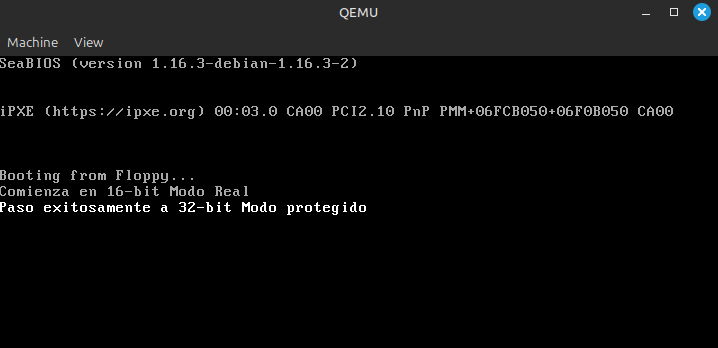
\includegraphics[width=0.8\textwidth]{images/switchtopm.png}
    \caption{Cambio de modo real a modo protegido funcionando.}
\end{figure}

\subsection{Programa con Descriptores de Código y Datos Diferenciados}

El Modo Protegido requiere definir explícitamente los segmentos de memoria que el programa utilizará a través de la GDT. Nuestro programa utiliza los descriptores mínimos necesarios para un funcionamiento básico:

\begin{itemize}
    \item \textbf{Descriptor Nulo (Índice 0):} Es obligatorio por la especificación Intel. Todos sus campos deben ser cero. Intentar cargar un selector que apunte a este descriptor causa una excepción.
    \item \textbf{Descriptor de Código (Índice 1, Selector 0x08):} Define las propiedades del segmento donde reside nuestro código ejecutable.
        \begin{itemize}
            \item \texttt{Base = 0x00000000}: El segmento empieza al inicio de la memoria física.
            \item \texttt{Límite = 0xFFFFF (con Granularidad=1)}: El segmento se extiende por 4 GiB (\( (0xFFFFF + 1) \times 4096 \)). Cubre todo el espacio de direcciones direccionable en 32 bits. Esto se conoce como modelo «plano» (flat model).
            \item \texttt{Acceso = 0x9A}: Indica que es un segmento Presente (P=1), de nivel de privilegio 0 (DPL=00, el más alto, Ring 0), de tipo Código (S=1, Type=1010), que es Ejecutable y Leíble (R=1).
            \item \texttt{Flags = 0xCF}: Indica Granularidad de 4KiB (G=1), tamaño de operando/dirección de 32 bits (D=1), y los bits altos del límite.
        \end{itemize}
        El registro \texttt{CS} se carga con el selector \texttt{0x08} mediante el \texttt{ljmp}.
    \item \textbf{Descriptor de Datos (Índice 2, Selector 0x10):} Define las propiedades del segmento para datos y la pila.
        \begin{itemize}
            \item \texttt{Base = 0x00000000}: Igual que el código, empieza al inicio de la memoria.
            \item \texttt{Límite = 0xFFFFF (con Granularidad=1)}: Igual, 4 GiB. Modelo plano.
            \item \texttt{Acceso = 0x92}: Indica Presente (P=1), DPL=00, de tipo Datos (S=1, Type=0010), que es Leíble y Escribible (W=1).
            \item \texttt{Flags = 0xCF}: Idéntico al segmento de código (32 bits, granularidad 4K).
        \end{itemize}
        Los registros \texttt{DS}, \texttt{ES}, \texttt{FS}, \texttt{GS}, \texttt{SS} se cargan con el selector \texttt{0x10} después de entrar en modo protegido.
\end{itemize}

\subsubsection{Espacios de Memoria Diferenciados (Concepto vs. Implementación Plana)}

La pregunta pide específicamente segmentos en «espacios de memoria diferenciados». Con los descriptores definidos arriba (modelo plano), tanto el código como los datos \textit{pueden} acceder teóricamente al mismo espacio lineal completo de 4 GiB porque ambos tienen Base=0 y Límite=4 GiB.

Para tener espacios verdaderamente \textit{diferenciados} y separados por hardware (más allá de solo los permisos R/W/X), necesitaríamos definir descriptores con \textbf{bases y/o límites diferentes}. Por ejemplo:

\begin{itemize}
    \item \textbf{Código Separado:} Se podría definir el descriptor de código con Base=0x100000 y Límite=0xFFFFF (cubriendo desde 1 MiB hasta 4 GiB+1 MiB con granularidad), mientras que el de datos tiene Base=0 y Límite=0x1FFFF (cubriendo los primeros 128 KiB con granularidad de byte para la pila y datos iniciales).
    \item \textbf{Datos Separados:} Podríamos tener Código Base=0, Límite=Y, y Datos Base=Y+1, Límite=Z.
\end{itemize}

Esto requeriría:
\begin{enumerate}
    \item Modificar las definiciones \texttt{dw base\_low, db base\_mid, db base\_high} y \texttt{dw limit\_low, db flags\_limit\_high} en \texttt{gdt.asm} para cada descriptor.
    \item Asegurarse de que el linker coloque el código y los datos en las regiones de memoria física correspondientes a esas bases definidas en los descriptores. Esto requeriría un script \texttt{link.ld} más complejo, definiendo secciones \texttt{.text} y \texttt{.data} con direcciones de carga (\texttt{AT}) diferentes y especificando sus direcciones virtuales (\texttt{. = direccion\_virtual}) correspondientes a las bases de los descriptores.
\end{enumerate}

Sin embargo, para la funcionalidad básica de este TP, el \textbf{modelo plano (Base=0, Límite=4 GB para ambos)} es mucho más simple de implementar y es el modelo predominante usado por los sistemas operativos modernos (que luego utilizan paginación para la separación y protección fina). Nuestro código actual, aunque no usa bases/límites diferentes, sí tiene descriptores funcionalmente distintos para código (Ejecutable/Leíble) y datos (Leíble/Escribible).

% --- INICIO DEL CONTENIDO A INCLUIR ---

\section{Prueba de Protección de Memoria (Segmento Read-Only)}

Una de las características fundamentales introducidas por el Modo Protegido es la capacidad del hardware para hacer cumplir permisos de acceso a los segmentos de memoria definidos en la GDT. Para verificar esto experimentalmente, modificamos nuestro bootloader para intentar escribir en un segmento de datos configurado como "solo lectura".

\subsection{Modificaciones al Código}

Se realizaron dos cambios principales:

\begin{enumerate}
    \item \textbf{Definición de Descriptor Read-Only en \texttt{gdt.asm}:}
          Se añadió un tercer descriptor de datos a la GDT (después del descriptor de código y el de datos R/W).
          Este nuevo descriptor, etiquetado como \texttt{gdt\_data\_ro}, se configuró con los mismos Base (0)
          y Límite (4 GiB) que los demás, pero con un \textbf{Byte de Acceso} específico: \texttt{0x90}.
  
          \begin{lstlisting}[style=NasmStyle,
            caption={Descriptor Read-Only en \texttt{gdt.asm}}, numbers=none]
  ; Descriptor 3: Datos Read-Only (Selector 0x18)
  gdt_data_ro:
      dw 0xFFFF                   ; Limite (0-15)
      dw 0x0000                   ; Base (0-15)
      db 0x00                     ; Base (16-23)
      db 0x90                     ; <<< Byte de Acceso (10010000b) >>>
                                  ; P=1, DPL=0, S=1(Datos), Type=0000 -> Writable=0
      db 0xCF                     ; Flags(G=1, D=1 -> 32 bit) + Limit(16-19)
      db 0x00                     ; Base (24-31)
  
  gdt_end:                        ; Etiqueta movida al final
          \end{lstlisting}
  
          El byte de acceso \texttt{0x90} (\texttt{10010000b}) indica explícitamente que el segmento
          está presente (P = 1), es para Ring 0 (DPL = 00), es un segmento de datos (S = 1) y,
          crucialmente, el bit \textbf{Writable (W) es 0}, marcándolo como solo lectura.
          La etiqueta \texttt{gdt\_end} se movió para asegurar que el tamaño de la GDT (usado por
          \texttt{lgdt}) incluyera este nuevo descriptor.  
          El selector correspondiente a este tercer descriptor (índice 3) es \texttt{0x18}.
  
    \item \textbf{Intento de Escritura en Modo Protegido (en
          \texttt{switch\_to\_pm.asm}\,)\,:} % <- escape en caption más abajo
          Dentro de la rutina \texttt{BEGIN\_PM} (que se ejecuta en modo protegido), después de imprimir el
          mensaje de bienvenida y verificar opcionalmente una escritura válida en el segmento R/W,
          se añadió el siguiente bloque para probar la protección:
  
          \begin{lstlisting}[style=NasmStyle,
            caption={Intento de escritura R/O en \texttt{switch\_to\_pm.asm}}, % <-  \_
            numbers=none]
          ; Prueba con segmento R/O (Selector 0x18)
          mov ax, 0x18                ; Cargar Selector Datos Read-Only
          mov ds, ax                  ; Actualizar DS para usar el segmento R/O
          
          mov dword [0x3000], 0xDEADBEEF ;  usando el segmento definido por DS (ahora R/O)
                                          ;  ESTO DEBE FALLAR.
          
          ;
  .write_protection_failed:            ; <- un solo \texttt{} era suficiente
          ; 
          mov edi, 0xb8000 + 320       ; 
          mov ax, 0x4f45               ; 'E' roja
          mov [edi], ax
          mov ax, 0x4f52               ; 'R' roja
          mov [edi+2], ax
          mov ax, 0x4f52               ; 'R' roja
          mov [edi+4], ax
  .hang_error:
          cli
          hlt
          jmp .hang_error
          \end{lstlisting}
  
          Este código primero carga el selector \texttt{0x18} en el registro de segmento \texttt{DS}.
          Luego intenta escribir el valor \texttt{0xDEADBEEF} en la dirección de memoria \texttt{0x3000}
          utilizando implícitamente el segmento apuntado por \texttt{DS}.  
          Se añadió también una sección \texttt{.write\_protection\_failed} que solo se alcanzaría si,
          por error, la protección no se activara.
  \end{enumerate}
  



\subsection{Ejecución y Resultados: ¿Qué Sucede?}

Tras recompilar y enlazar el código con las modificaciones, se ejecutó la imagen \texttt{pm\_final.img} resultante. El comportamiento observado dependió del entorno de ejecución:

\begin{itemize}
    \item \textbf{En QEMU (modo TCG por defecto):}
          Al ejecutar \verb|qemu-system-i386 -fda pm_final.img -boot a| se observó lo siguiente:
  \begin{verbatim}
  Booting from Floppy...
  Comienza en 16-bit Modo Real
  Paso exitosamente a 32-bit Modo protegido
  ERR
  \end{verbatim}
  
          La aparición del mensaje \texttt{ERR} indica que la instrucción
          \verb|mov dword [0x3000], 0xDEADBEEF|
          \emph{no generó la excepción esperada}; la ejecución alcanzó el
          manejador de error \texttt{.write\_protection\_failed}.
          Esto se debe a una limitación de QEMU en modo TCG, que no realiza todas
          las comprobaciones de permisos R/W de los descriptores de segmento.
  
    \item \textbf{En Bochs (emulador preciso):}
          Al lanzar la misma imagen con \verb|bochs -q| (usando un \texttt{.bochsrc}
          adecuado) el comportamiento cambió:
          \begin{enumerate}[label=(\alph*)]
            \item Se mostraron los mensajes iniciales 
            \item La emulación se detuvo de inmediato.
            \item El log \texttt{bochsout.txt} registró:
  \begin{verbatim}
  ... (estado de registros justo antes del fallo) ...
  00XXX[CPU0 ] exception(): 3rd (13) exception with no resolution,
                shutdown status is 00h, resetting
  ... (mensajes de reinicio) ...
  \end{verbatim}
                  Bochs reportó la \textbf{excepción 13} (GP – General Protection Fault);
                  al no haber IDT pasó a triple falta y reinició la VM.
          \end{enumerate}
  
    \item \textbf{En QEMU con KVM:}
          Ejecutando \verb|qemu-system-i386 -enable-kvm -fda pm_final.img -boot a|
          se ven los dos mensajes iniciales y QEMU se cierra abruptamente: de nuevo
          se trata de la triple falta, que KVM/QEMU resuelve terminando la emulación.
  \end{itemize}
  

**Conclusión del Experimento:** La ejecución en Bochs y QEMU con KVM **verifica exitosamente** que la CPU (real o emulada con precisión) detecta el intento de escritura en un segmento marcado como Read-Only (W=0 en el descriptor) y genera la excepción de Falla de Protección General (GP) como se espera según la arquitectura x86.

\subsection{¿Qué Debería Suceder a Continuación (Teoría del Fallo)?}

Cuando la CPU ejecuta una instrucción que viola las reglas de protección definidas por los descriptores de segmento (como intentar escribir en un segmento R/O), ocurre la siguiente secuencia teórica:
\begin{enumerate}
    \item \textbf{Generación de Excepción GP (Vector 13):} La CPU detiene la ejecución de la instrucción infractora y genera una Falla de Protección General. Busca en la Tabla de Descriptores de Interrupción (IDT) la entrada correspondiente al vector 13.
    \item \textbf{Intento de Invocar al Manejador GP:} La CPU intenta transferir el control al manejador de excepciones definido en la entrada 13 de la IDT.
    \item \textbf{Fallo por Falta de IDT/Manejador (Doble Falta):} En nuestro bootloader, no hemos configurado ni cargado una IDT para el Modo Protegido usando la instrucción \texttt{lidt}. La CPU no encuentra un descriptor válido para el vector 13. Este fallo al manejar una excepción genera una nueva excepción: la **Doble Falta (Excepción DF - Vector 8)**.
    \item \textbf{Intento de Invocar al Manejador DF:} La CPU intenta transferir el control al manejador de Doble Falta definido en la entrada 8 de la IDT.
    \item \textbf{Fallo por Falta de Manejador DF (Triple Falta):} Como sigue sin haber una IDT válida, la CPU falla de nuevo al intentar manejar la Doble Falta. Una excepción ocurrida mientras se intenta invocar al manejador de Doble Falta resulta en una condición irrecuperable conocida como **Triple Falta**.
    \item \textbf{Shutdown (Apagado/Reinicio):} Ante una Triple Falta, la CPU entra en un estado de "shutdown". En hardware real, esto generalmente provoca un reinicio inmediato de la placa base. Los emuladores como Bochs y QEMU+KVM simulan este comportamiento deteniendo la emulación o reportando el fallo fatal.
\end{enumerate}
Por lo tanto, el resultado esperado al intentar escribir en el segmento R/O en nuestro contexto (sin IDT) es, efectivamente, un Triple Fallo que detiene o reinicia el sistema.

\subsection{Verificación con GDB}

Aunque QEMU en modo TCG no genera el GP, GDB sigue siendo útil para verificar que los prerrequisitos para el fallo *estaban* presentes:
\begin{enumerate}
    \item Se conectó GDB a QEMU (`target remote`).
    \item Se cargó el archivo ELF (`file pm.elf`) para obtener símbolos (aunque GDB mostró advertencias, pudo usarlos parcialmente).
    \item Se establecieron las arquitecturas correctas (`set architecture i8086` / `set architecture i386`).
    \item Se verificó la GDT en memoria antes de `lgdt` usando `x/32bx 'direccion\_gdt\_start'`, confirmando que el tercer descriptor tenía el byte de acceso \texttt{0x90}.
    \item Se avanzó la ejecución hasta justo antes de la instrucción \texttt{mov dword [0x3000], 0xDEADBEEF}.
    \item Se verificó con \texttt{info registers ds} que el registro \texttt{DS} contenía correctamente el selector \texttt{0x18}.
    \item Al ejecutar \texttt{si} sobre la instrucción de escritura, se observó que GDB avanzaba a la siguiente instrucción (llevando a "ERR") en lugar de reportar \texttt{SIGSEGV / General Protection Fault}.
\end{enumerate}

Esta depuración confirma que el código cargó el selector correcto para el segmento R/O, pero la excepción no fue generada por el entorno de emulación TCG. Si se hubiera depurado bajo Bochs o KVM, el último \texttt{si} habría mostrado la recepción de la señal \texttt{SIGSEGV}.

\subsection{Valor y Propósito de los Selectores en Modo Protegido}

\textbf{Pregunta:} En modo protegido, ¿Con qué valor se cargan los registros de segmento? ¿Porque?

\textbf{Respuesta:}
En Modo Protegido, los registros de segmento (CS, DS, ES, SS, FS, GS) **NO** se cargan con direcciones base como en Modo Real. En su lugar, se cargan con valores de 16 bits llamados **Selectores**. En nuestro ejemplo, DS, ES, SS, etc., se cargaron con el selector \texttt{0x10} para el segmento de datos R/W, y luego DS se cambió al selector \texttt{0x18} para el segmento R/O.

La estructura de un selector es:
\begin{itemize}[noitemsep]
    \item \textbf{Bits 15-3 (13 bits): Índice.} Especifica el número de entrada (descriptor) a utilizar dentro de una tabla de descriptores.
    \item \textbf{Bit 2 (TI - Table Indicator):} Indica si se usa la GDT (TI=0) o la LDT (TI=1). Nuestros selectores 0x08, 0x10, 0x18 tienen TI=0.
    \item \textbf{Bits 1-0 (RPL - Requested Privilege Level):} Indica el nivel de privilegio solicitado para la operación. Generalmente es 0 para código de kernel. Nuestros selectores tienen RPL=0.
\end{itemize}
Por ejemplo, el selector \texttt{0x18} (binario \texttt{0000000000011000}) tiene: Índice = 3, TI = 0 (GDT), RPL = 0.

**¿Por qué se usan Selectores en lugar de direcciones base?**

Este mecanismo de indirección es fundamental para las características clave del Modo Protegido:
\begin{enumerate}
    \item \textbf{Protección de Memoria:} Cuando se realiza un acceso a memoria (ej. leer de \texttt{DS:[offset]}), la CPU no usa directamente el valor en DS. Utiliza el \textit{selector} en DS para buscar el \textit{descriptor} correspondiente en la GDT. Este descriptor contiene la dirección base real, el límite del segmento y los bits de permiso (R/W/X, DPL). La CPU realiza comprobaciones automáticas por hardware: ¿Está el \texttt{offset} dentro del \texttt{límite}? ¿Permite el descriptor la operación (lectura/escritura)? ¿Tiene el código actual (CPL) y el selector (RPL) suficientes privilegios para acceder a un segmento con este DPL? Si alguna comprobación falla, se genera una excepción (GP, SS). Esto impide que un programa acceda o corrompa memoria fuera de sus segmentos asignados o con permisos insuficientes.
    \item \textbf{Niveles de Privilegio (Rings):} Los campos DPL (en el descriptor) y CPL/RPL (en CS/selector) permiten implementar anillos de protección, donde el código del sistema operativo (Ring 0) está protegido de las aplicaciones de usuario (Ring 3).
    \item \textbf{Flexibilidad y Memoria Virtual:} Permite al sistema operativo reubicar segmentos en la memoria física simplemente actualizando sus descriptores en la GDT, sin necesidad de cambiar el código que usa los selectores. También se integra con el sistema de paginación para implementar memoria virtual compleja.
\end{enumerate}
En esencia, los selectores y descriptores trasladan la responsabilidad de la gestión y protección de la memoria del software (como en Modo Real) al hardware de la CPU, proporcionando una base mucho más robusta y segura para los sistemas operativos modernos.


